\section{Реализация}

\subsection{Архитектура приложения}

Приложение «Телефонный справочник» построено на основе объектно-ориентированного подхода с четким разделением ответственности между компонентами системы. Архитектура следует принципам модульности и слабой связанности, что обеспечивает удобство сопровождения и расширения функциональности.

Основные компоненты приложения:
\begin{itemize}
    \item \textbf{Contact} — структура данных для хранения информации о контакте;
    \item \textbf{ContactValidator} — класс для валидации и нормализации пользовательского ввода;
    \item \textbf{ContactStorage} — класс для работы с файловым хранилищем (JSON);
    \item \textbf{MainWindow} — класс главного окна, реализующий графический интерфейс и логику взаимодействия с пользователем.
\end{itemize}

Структура директорий проекта:

\begin{lstlisting}[style=cstyle, style=cstyle, caption={Структура проекта}]
lab8/
├── CMakeLists.txt
├── src/
│   ├── main.cpp
│   ├── contact.cpp
│   ├── contactstorage.cpp
│   ├── contactvalidator.cpp
│   └── mainwindow.cpp
└── headers/
    ├── contact.h
    ├── contactstorage.h
    ├── contactvalidator.h
    └── mainwindow.h
\end{lstlisting}

Взаимодействие компонентов представлено на диаграмме (см. рисунок~\ref{fig:architecture}).

\begin{figure}[H]
    \centering
    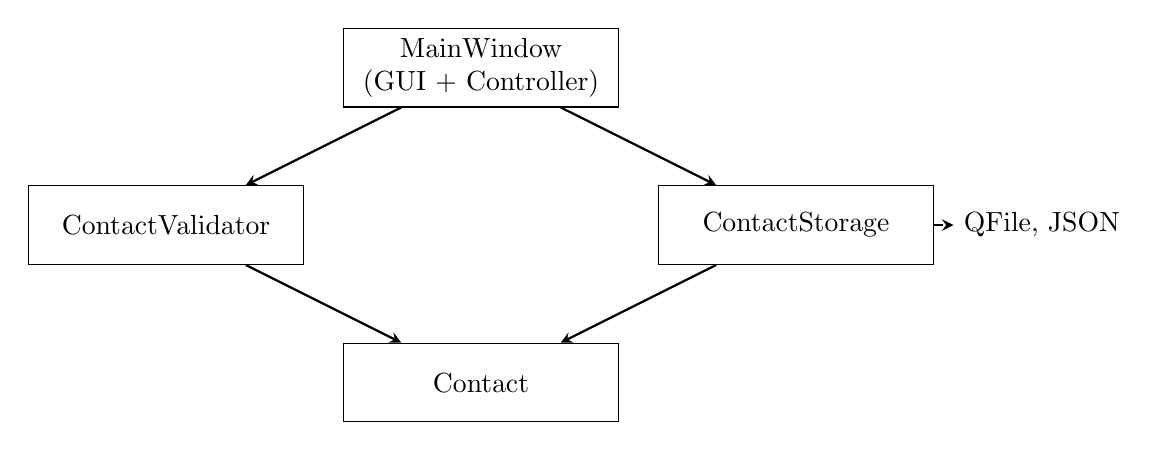
\begin{tikzpicture}[
        box/.style={rectangle, draw, minimum width=3.5cm, minimum height=1cm, align=center},
        arrow/.style={->, >=stealth, thick}
    ]
        \node[box] (mainwindow) at (0,4) {MainWindow\\(GUI + Controller)};
        \node[box] (validator) at (-4,2) {ContactValidator};
        \node[box] (storage) at (4,2) {ContactStorage};
        \node[box] (contact) at (0,0) {Contact};
        
        \draw[arrow] (mainwindow) -- (validator);
        \draw[arrow] (mainwindow) -- (storage);
        \draw[arrow] (storage) -- (contact);
        \draw[arrow] (validator) -- (contact);
        \draw[arrow, dashed] (storage) -- ++(2,0) node[right] {QFile, JSON};
    \end{tikzpicture}
    \caption{Архитектура приложения}
    \label{fig:architecture}
\end{figure}

Класс \texttt{MainWindow} выступает центральным компонентом, координирующим работу остальных модулей. Он обрабатывает события пользовательского интерфейса, вызывает методы валидации перед операциями с данными и использует \texttt{ContactStorage} для сохранения и загрузки информации.

\subsection{Описание классов}

\subsubsection{Структура Contact}

Структура \texttt{Contact} представляет модель данных для хранения информации о контакте. Содержит все необходимые поля согласно требованиям задания.

\begin{lstlisting}[style=cstyle, style=cstyle, caption={Заголовочный файл contact.h}]
#ifndef CONTACT_H
#define CONTACT_H

#include <QString>
#include <QDate>
#include <QStringList>
#include <QJsonObject>

class Contact
{
public:
    Contact();
    Contact(const QString& firstName, const QString& lastName, 
            const QString& middleName, const QString& address, 
            const QDate& birthDate, const QString& email,
            const QStringList& phoneNumbers);

    QString firstName() const { return m_firstName; }
    QString lastName() const { return m_lastName; }
    QString middleName() const { return m_middleName; }
    QString address() const { return m_address; }
    QDate birthDate() const { return m_birthDate; }
    QString email() const { return m_email; }
    QStringList phoneNumbers() const { return m_phoneNumbers; }

    void setFirstName(const QString& firstName);
    void setLastName(const QString& lastName);
    void setMiddleName(const QString& middleName);
    void setAddress(const QString& address);
    void setBirthDate(const QDate& birthDate);
    void setEmail(const QString& email);
    void setPhoneNumbers(const QStringList& phoneNumbers);

    QJsonObject toJson() const;
    static Contact fromJson(const QJsonObject& json);

    bool operator<(const Contact& other) const;
    bool operator==(const Contact& other) const;

private:
    QString m_firstName;
    QString m_lastName;
    QString m_middleName;
    QString m_address;
    QDate m_birthDate;
    QString m_email;
    QStringList m_phoneNumbers;
};

#endif // CONTACT_H
\end{lstlisting}

Класс реализует методы сериализации в формат JSON и десериализации из него, что обеспечивает удобное сохранение данных в файл. Операторы сравнения используются для сортировки контактов по фамилии, имени и отчеству.

\subsubsection{Класс ContactValidator}

Класс \texttt{ContactValidator} инкапсулирует логику валидации пользовательского ввода с использованием регулярных выражений. Обеспечивает проверку корректности данных перед их сохранением.

\begin{lstlisting}[style=cstyle, caption={Заголовочный файл contactvalidator.h}]
#ifndef CONTACTVALIDATOR_H
#define CONTACTVALIDATOR_H

#include <QString>
#include <QDate>

class ContactValidator
{
public:
    static bool validateName(const QString& name, 
                             QString& errorMessage);
    static bool validatePhone(const QString& phone, 
                              QString& errorMessage);
    static bool validateBirthDate(const QDate& date, 
                                  QString& errorMessage);
    static bool validateEmail(const QString& email, 
                             QString& errorMessage);

    // Методы нормализации
    static QString normalizeName(const QString& name);
    static QString normalizePhone(const QString& phone);
    static QString normalizeEmail(const QString& email);

private:
    static QString extractPhoneDigits(const QString& phone);
};

#endif // CONTACTVALIDATOR_H
\end{lstlisting}

\textbf{Регулярные выражения для валидации:}

\begin{itemize}
    \item \textbf{Имя:} \texttt{\^{}[A-Za-zА-Яа-яЁё0-9][A-Za-zА-Яа-яЁё0-9\textbackslash- ]*[A-Za-zА-Яа-яЁё0-9]\$}
    \begin{itemize}
        \item Разрешены буквы (латиница и кириллица), цифры, дефис, пробел;
        \item Не может начинаться или заканчиваться дефисом;
        \item Запрещены двойные дефисы и множественные пробелы.
    \end{itemize}
    
    \item \textbf{Телефон:} \texttt{\^{}\textbackslash+\textbackslash d+\$}
    \begin{itemize}
        \item Международный формат (начинается с +);
        \item Длина от 10 до 15 цифр;
        \item Автоматическое преобразование формата 8(XXX)XXX-XX-XX в +7XXXXXXXXXX.
    \end{itemize}
    
    \item \textbf{Email:} \texttt{\^{}[A-Za-z0-9.\_\%+-]+@[A-Za-z0-9.-]+\textbackslash.[A-Za-z]\{2,\}\$}
    \begin{itemize}
        \item Имя пользователя: латинские буквы, цифры, точки, подчеркивания;
        \item Обязательное наличие символа @;
        \item Домен должен содержать минимум одну точку.
    \end{itemize}
    
    \item \textbf{Дата рождения:}
    \begin{itemize}
        \item Должна быть меньше текущей даты;
        \item Не может быть более 150 лет назад;
        \item Валидация високосных годов выполняется классом QDate.
    \end{itemize}
\end{itemize}

\textbf{Псевдокод метода validateName:}

\begin{quote}
\textbf{Функция validateName(name, errorMessage):} \\
\hspace*{1em}normalized = normalizeName(name) \\
\hspace*{1em}если normalized пусто: \\
\hspace*{2em}errorMessage = "Имя не может быть пустым" \\
\hspace*{2em}вернуть false \\
\hspace*{1em}trimmed = name.trimmed() \\
\hspace*{1em}если trimmed начинается или заканчивается на '-': \\
\hspace*{2em}errorMessage = "Имя не может начинаться/заканчиваться на дефис" \\
\hspace*{2em}вернуть false \\
\hspace*{1em}regex = \^{}[A-Za-zА-Яа-яЁё0-9][A-Za-zА-Яа-яЁё0-9\textbackslash- ]*[A-Za-zА-Яа-яЁё0-9]\$ \\
\hspace*{1em}если не соответствует regex: \\
\hspace*{2em}errorMessage = "Имя может содержать только буквы, цифры, дефис и пробел" \\
\hspace*{2em}вернуть false \\
\hspace*{1em}если содержит "--" или множественные пробелы: \\
\hspace*{2em}errorMessage = "Имя не должно содержать двойные дефисы или множественные пробелы" \\
\hspace*{2em}вернуть false \\
\hspace*{1em}вернуть true
\end{quote}

\textbf{Методы нормализации:}

Нормализация обеспечивает приведение данных к единому формату перед сохранением:

\begin{itemize}
    \item \texttt{normalizeName} — удаляет лишние пробелы, приводит первую букву каждого слова к заглавной, остальные к строчным;
    \item \texttt{normalizePhone} — удаляет пробелы, скобки, дефисы, преобразует российский формат 8(...) в +7(...);
    \item \texttt{normalizeEmail} — приводит к нижнему регистру, удаляет пробелы.
\end{itemize}

\subsubsection{Класс ContactStorage}

Класс \texttt{ContactStorage} отвечает за сохранение и загрузку контактов из файла в формате JSON. Использует классы \texttt{QFile}, \texttt{QJsonDocument}, \texttt{QJsonArray} и \texttt{QJsonObject} из фреймворка Qt.

\begin{lstlisting}[style=cstyle, caption={Заголовочный файл contactstorage.h}]
#ifndef CONTACTSTORAGE_H
#define CONTACTSTORAGE_H

#include "contact.h"
#include <QList>
#include <QString>

class ContactStorage
{
public:
    ContactStorage(const QString& filename = "phonebook.json");
    
    bool load();
    bool save();
    
    QList<Contact>& contacts();
    const QList<Contact>& contacts() const;
    
    void addContact(const Contact& contact);
    void removeContact(int index);
    void updateContact(int index, const Contact& contact);
    
    QString filename() const;
    void setFilename(const QString& filename);

private:
    QList<Contact> m_contacts;
    QString m_filename;
};

#endif // CONTACTSTORAGE_H
\end{lstlisting}

\textbf{Псевдокод метода load:}

\begin{quote}
\textbf{Функция load():} \\
\hspace*{1em}file = открыть m\_filename для чтения \\
\hspace*{1em}если файл не существует: \\
\hspace*{2em}m\_contacts.clear() \\
\hspace*{2em}вернуть true \\
\hspace*{1em}если не удалось открыть файл: \\
\hspace*{2em}вывести ошибку \\
\hspace*{2em}вернуть false \\
\hspace*{1em}data = прочитать весь файл \\
\hspace*{1em}закрыть файл \\
\hspace*{1em}doc = разобрать data как JSON \\
\hspace*{1em}если ошибка парсинга: \\
\hspace*{2em}вывести ошибку \\
\hspace*{2em}вернуть false \\
\hspace*{1em}если doc не является массивом: \\
\hspace*{2em}вывести ошибку \\
\hspace*{2em}вернуть false \\
\hspace*{1em}array = doc.array() \\
\hspace*{1em}m\_contacts.clear() \\
\hspace*{1em}для каждого value в array: \\
\hspace*{2em}если value является объектом: \\
\hspace*{3em}contact = Contact::fromJson(value) \\
\hspace*{3em}m\_contacts.append(contact) \\
\hspace*{1em}вернуть true
\end{quote}

\textbf{Псевдокод метода save:}

\begin{quote}
\textbf{Функция save():} \\
\hspace*{1em}file = открыть m\_filename для записи \\
\hspace*{1em}если не удалось открыть файл: \\
\hspace*{2em}вывести ошибку \\
\hspace*{2em}вернуть false \\
\hspace*{1em}array = пустой JSON-массив \\
\hspace*{1em}для каждого contact в m\_contacts: \\
\hspace*{2em}jsonObject = contact.toJson() \\
\hspace*{2em}array.append(jsonObject) \\
\hspace*{1em}doc = QJsonDocument(array) \\
\hspace*{1em}записать doc.toJson() в файл \\
\hspace*{1em}закрыть файл \\
\hspace*{1em}вернуть true
\end{quote}


\subsubsection{Класс MainWindow}

Класс \texttt{MainWindow} наследуется от \texttt{QMainWindow} и реализует графический интерфейс приложения, а также всю бизнес-логику взаимодействия с пользователем.

\begin{lstlisting}[style=cstyle, caption={Фрагмент заголовочного файла mainwindow.h}]
#ifndef MAINWINDOW_H
#define MAINWINDOW_H

#include <QMainWindow>
#include <QTableWidget>
#include <QPushButton>
#include <QLineEdit>
#include <QDateEdit>
#include <QTextEdit>
#include <QComboBox>
#include <QStack>
#include "contactstorage.h"
#include "contact.h"

struct ContactAction {
    enum Type { Add, Edit, Delete };
    Type type;
    Contact contact;
    int index;
};

class MainWindow : public QMainWindow
{
    Q_OBJECT

public:
    MainWindow(QWidget *parent = nullptr);
    ~MainWindow();

private slots:
    void addContact();
    void editContact();
    void deleteContact();
    void searchContacts();
    void clearSearch();
    void onTableSelectionChanged();
    void loadContacts();
    void saveContacts();
    void undoLastAction();

private:
    void setupUI();
    void setupTable();
    void setupForm();
    void setupSearch();
    void populateTable();
    void clearForm();
    bool validateForm(QString& errorMessage);
    bool checkForDuplicates(const Contact& contact, 
                           int excludeIndex = -1);
    
    // UI компоненты
    QTableWidget* m_table;
    QLineEdit* m_firstNameEdit;
    QLineEdit* m_lastNameEdit;
    QLineEdit* m_middleNameEdit;
    QTextEdit* m_addressEdit;
    QDateEdit* m_birthDateEdit;
    QLineEdit* m_emailEdit;
    QTextEdit* m_phoneNumbersEdit;
    QPushButton* m_addButton;
    QPushButton* m_editButton;
    QPushButton* m_deleteButton;
    QPushButton* m_undoButton;
    QLineEdit* m_searchEdit;
    QComboBox* m_searchFieldCombo;
    QDateEdit* m_searchDateEdit;
    QComboBox* m_dateSearchTypeCombo;
    
    // Данные
    ContactStorage* m_storage;
    int m_editingIndex;
    bool m_isEditing;
    QStack<ContactAction> m_undoStack;
};

#endif // MAINWINDOW_H
\end{lstlisting}

\textbf{Ключевые компоненты графического интерфейса:}

\begin{itemize}
    \item \textbf{QTableWidget} — таблица для отображения контактов с возможностью сортировки по столбцам;
    \item \textbf{QLineEdit, QTextEdit, QDateEdit} — поля ввода данных контакта;
    \item \textbf{QComboBox} — выпадающие списки для выбора поля поиска и типа сравнения даты;
    \item \textbf{QPushButton} — кнопки управления (Добавить, Редактировать, Удалить, Отмена, Поиск);
    \item \textbf{QGroupBox} — группировка элементов формы и поиска.
\end{itemize}

Внешний вид главного окна представлен на рисунке~\ref{fig:main_window}.
% TODO: вставить скриншот
\begin{figure}[H]
    \centering
    % \includegraphics[width=1\linewidth]{myPhoto/main_window.png}
    \caption{Главное окно приложения}
    \label{fig:main_window}
\end{figure}

\textbf{Механизм сигналов и слотов:}

Qt использует архитектуру сигналов и слотов для обработки событий. Основные соединения в приложении:
% TODO: русский язык
\begin{lstlisting}[style=cstyle, caption={Соединения сигналов и слотов}]
// Кнопки управления
connect(m_addButton, &QPushButton::clicked, 
        this, &MainWindow::addContact);
connect(m_editButton, &QPushButton::clicked, 
        this, &MainWindow::editContact);
connect(m_deleteButton, &QPushButton::clicked, 
        this, &MainWindow::deleteContact);
connect(m_undoButton, &QPushButton::clicked, 
        this, &MainWindow::undoLastAction);

// Поиск
connect(m_searchButton, &QPushButton::clicked, 
        this, &MainWindow::searchContacts);
connect(m_clearSearchButton, &QPushButton::clicked, 
        this, &MainWindow::clearSearch);

// Таблица
connect(m_table, &QTableWidget::itemSelectionChanged, 
        this, &MainWindow::onTableSelectionChanged);

// Автосохранение
connect(m_storage, &ContactStorage::dataChanged, 
        this, &MainWindow::saveContacts);
\end{lstlisting}

\subsection{Ключевые алгоритмы}

\subsubsection{Алгоритм добавления контакта}

Процесс добавления нового контакта включает несколько этапов проверки и обработки данных. Псевдокод представлен ниже.

\textbf{Псевдокод метода addContact:}

\begin{quote}
\textbf{Функция addContact():} \\
\hspace*{1em}errorMessage = "" \\
\hspace*{1em}если не validateForm(errorMessage): \\
\hspace*{2em}показать диалог с ошибкой errorMessage \\
\hspace*{2em}вернуться \\
\hspace*{1em}contact = получить данные из формы \\
\hspace*{1em}если m\_isEditing == true: \\
\hspace*{2em}oldContact = m\_storage.contacts()[m\_editingIndex] \\
\hspace*{2em}если checkForDuplicates(contact, m\_editingIndex): \\
\hspace*{3em}показать диалог "Такой контакт уже существует" \\
\hspace*{3em}вернуться \\
\hspace*{2em}m\_storage.updateContact(m\_editingIndex, contact) \\
\hspace*{2em}pushAction(Edit, oldContact, m\_editingIndex) \\
\hspace*{2em}показать сообщение "Контакт обновлен" \\
\hspace*{2em}m\_isEditing = false \\
\hspace*{2em}m\_addButton.setText("Добавить") \\
\hspace*{1em}иначе: \\
\hspace*{2em}если checkForDuplicates(contact): \\
\hspace*{3em}показать предупреждение о дубликате \\
\hspace*{3em}если пользователь отменил: \\
\hspace*{4em}вернуться \\
\hspace*{2em}m\_storage.addContact(contact) \\
\hspace*{2em}pushAction(Add, contact, m\_storage.contactCount() - 1) \\
\hspace*{2em}показать сообщение "Контакт добавлен" \\
\hspace*{1em}m\_storage.save() \\
\hspace*{1em}populateTable() \\
\hspace*{1em}clearForm()
\end{quote}

\subsubsection{Алгоритм поиска контактов}

Приложение поддерживает два типа поиска:
\begin{itemize}
    \item \textbf{Поиск по текстовым полям} (имя, фамилия, отчество, email, телефон, адрес) — поиск подстроки без учета регистра;
    \item \textbf{Поиск по дате рождения} — точное совпадение, диапазон "до даты", "после даты".
\end{itemize}

\textbf{Псевдокод метода searchContacts:}

\begin{quote}
\textbf{Функция searchContacts():} \\
\hspace*{1em}searchField = m\_searchFieldCombo.currentText() \\
\hspace*{1em}m\_table.clearContents() \\
\hspace*{1em}m\_table.setRowCount(0) \\
\hspace*{1em}row = 0 \\
\hspace*{1em}если searchField == "Дата рождения": \\
\hspace*{2em}searchDate = m\_searchDateEdit.date() \\
\hspace*{2em}searchType = m\_dateSearchTypeCombo.currentText() \\
\hspace*{2em}для каждого contact в m\_storage.contacts(): \\
\hspace*{3em}match = false \\
\hspace*{3em}если searchType == "Точное совпадение" и contact.birthDate() == searchDate: \\
\hspace*{4em}match = true \\
\hspace*{3em}если searchType == "До даты" и contact.birthDate() <= searchDate: \\
\hspace*{4em}match = true \\
\hspace*{3em}если searchType == "После даты" и contact.birthDate() >= searchDate: \\
\hspace*{4em}match = true \\
\hspace*{3em}если match: \\
\hspace*{4em}добавить contact в таблицу, строка row \\
\hspace*{4em}row = row + 1 \\
\hspace*{1em}иначе: \\
\hspace*{2em}searchText = m\_searchEdit.text().toLower() \\
\hspace*{2em}для каждого contact в m\_storage.contacts(): \\
\hspace*{3em}value = получить значение поля searchField из contact \\
\hspace*{3em}если value содержит searchText (без учета регистра): \\
\hspace*{4em}добавить contact в таблицу, строка row \\
\hspace*{4em}row = row + 1 \\
\hspace*{1em}если row == 0: \\
\hspace*{2em}показать сообщение "Ничего не найдено"
\end{quote}

\subsubsection{Механизм отмены действий}

Для реализации функции отмены последнего действия используется структура \texttt{ContactAction} и стек \texttt{QStack<ContactAction>}.

\textbf{Структура ContactAction:}
\begin{lstlisting}[style=cstyle, caption={Структура для хранения действия}]
struct ContactAction {
    enum Type { Add, Edit, Delete };
    Type type;         // Тип действия
    Contact contact;   // Сохраненный контакт
    int index;         // Индекс (для Edit и Delete)
};
\end{lstlisting}

\textbf{Псевдокод метода undoLastAction:}

\begin{quote}
\textbf{Функция undoLastAction():} \\
\hspace*{1em}если m\_undoStack пуст: \\
\hspace*{2em}показать сообщение "Нечего отменять" \\
\hspace*{2em}вернуться \\
\hspace*{1em}action = m\_undoStack.pop() \\
\hspace*{1em}если action.type == Add: \\
\hspace*{2em}m\_storage.removeContact(action.index) \\
\hspace*{2em}показать сообщение "Добавление отменено" \\
\hspace*{1em}если action.type == Edit: \\
\hspace*{2em}m\_storage.updateContact(action.index, action.contact) \\
\hspace*{2em}показать сообщение "Редактирование отменено" \\
\hspace*{1em}если action.type == Delete: \\
\hspace*{2em}m\_storage.contacts().insert(action.index, action.contact) \\
\hspace*{2em}показать сообщение "Удаление отменено" \\
\hspace*{1em}m\_storage.save() \\
\hspace*{1em}populateTable() \\
\hspace*{1em}clearForm()
\end{quote}

При каждом изменении данных (добавление, редактирование, удаление) информация о действии сохраняется в стек методом \texttt{pushAction}. Это позволяет откатить последнюю операцию одним нажатием кнопки "Отменить".

\subsubsection{Проверка на дубликаты}

Перед добавлением или редактированием контакта выполняется проверка на наличие идентичных записей. Контакты считаются дубликатами, если совпадают все поля, кроме списка телефонов.

\textbf{Псевдокод метода checkForDuplicates:}

\begin{quote}
\textbf{Функция checkForDuplicates(contact, excludeIndex):} \\
\hspace*{1em}для i от 0 до m\_storage.contactCount() - 1: \\
\hspace*{2em}если i == excludeIndex: \\
\hspace*{3em}продолжить следующую итерацию \\
\hspace*{2em}existing = m\_storage.contacts()[i] \\
\hspace*{2em}если existing.firstName() == contact.firstName() и \\
\hspace*{2em}\hspace*{2em}existing.lastName() == contact.lastName() и \\
\hspace*{2em}\hspace*{2em}existing.middleName() == contact.middleName() и \\
\hspace*{2em}\hspace*{2em}existing.birthDate() == contact.birthDate() и \\
\hspace*{2em}\hspace*{2em}existing.email() == contact.email() и \\
\hspace*{2em}\hspace*{2em}existing.address() == contact.address(): \\
\hspace*{3em}вернуть true \\
\hspace*{1em}вернуть false
\end{quote}

Если обнаружен дубликат, пользователю выводится п��едупреждение с вопросом о продолжении добавления.

\subsection{Сортировка данных}

Сортировка контактов в таблице выполняется автоматически при клике на заголовок столбца благодаря встроенному механизму \texttt{QTableWidget}. Метод \texttt{setSortingEnabled(true)} активирует эту функциональность.

При каждой загрузке данных из файла список контактов предварительно сортируется по фамилии, имени и отчеству с помощью оператора \texttt{operator<}, реализованного в классе \texttt{Contact}:

\begin{lstlisting}[style=cstyle, caption={Оператор сравнения для сортировки}]
bool Contact::operator<(const Contact& other) const
{
    if (m_lastName != other.m_lastName) {
        return m_lastName < other.m_lastName;
    }
    if (m_firstName != other.m_firstName) {
        return m_firstName < other.m_firstName;
    }
    return m_middleName < other.m_middleName;
}
\end{lstlisting}

Данный подход обеспечивает единообразие отображения данных при каждом запуске приложения.

\newpage

\section{Тестирование приложения}

В данном разделе представлены основные сценарии использования приложения с описанием действий пользователя и ожидаемого поведения системы.

\subsection{Начальное состояние приложения}

При первом запуске приложения отображается главное окно с пустой таблицей контактов и формой ввода данных. Если файл \texttt{phonebook.json} не существует, он будет автоматически создан при сохранении первого контакта.

\begin{figure}[H]
    \centering
    % \includegraphics[width=1\linewidth]{myPhoto/first_start.png}
    \caption{Начальное состояние приложения при первом запуске}
    \label{fig:first_start}
\end{figure}

Элементы интерфейса:
\begin{itemize}
    \item \textbf{Форма ввода данных} — содержит поля для всех атрибутов контакта;
    \item \textbf{Кнопки управления} — "Добавить", "Редактировать", "Удалить", "Отменить";
    \item \textbf{Панель поиска} — поле ввода, выбор поля для поиска, фильтры по дате;
    \item \textbf{Таблица контактов} — отображает список всех записей с возможностью сортировки;
    \item \textbf{Кнопки файловых операций} — "Сохранить" и "Загрузить".
\end{itemize}

\subsection{Сценарий 1: Добавление нового контакта}

\subsubsection{Шаг 1: Заполнение формы}

Пользователь заполняет все поля формы корректными данными:

\begin{itemize}
    \item \textbf{Фамилия:} Иванов
    \item \textbf{Имя:} Иван
    \item \textbf{Отчество:} Иванович
    \item \textbf{Адрес:} г. Москва, ул. Ленина, д. 1, кв. 10
    \item \textbf{Дата рождения:} 15.03.1990 (выбор через календарь)
    \item \textbf{Email:} ivan.ivanov@example.com
    \item \textbf{Телефоны:} +7 (999) 123-45-67, 8-800-555-35-35
\end{itemize}

\begin{figure}[H]
    \centering
    % \includegraphics[width=1\linewidth]{myPhoto/add_form_filled.png}
    \caption{Заполненная форма для добавления контакта}
    \label{fig:add_form_filled}
\end{figure}

\subsubsection{Шаг 2: Нормализация данных}

При вводе данных класс \texttt{ContactValidator} автоматически нормализует некоторые поля:

\begin{itemize}
    \item \textbf{Имя "иван"} преобразуется в \textbf{"Иван"} (первая буква заглавная);
    \item \textbf{Телефон "8-800-555-35-35"} преобразуется в \textbf{"+78005553535"} (международный формат);
    \item \textbf{Email "Ivan.Ivanov@Example.COM"} преобразуется в \textbf{"ivan.ivanov@example.com"} (нижний регистр).
\end{itemize}

Если происходит нормализация, пользователю выводится предупреждение с указанием изменений (см. рисунок~\ref{fig:format_warning}).

\begin{figure}[H]
    \centering
    % \includegraphics[width=0.8\linewidth]{myPhoto/format_warning.png}
    \caption{Предупреждение о нормализации данных}
    \label{fig:format_warning}
\end{figure}

\subsubsection{Шаг 3: Успешное добавление}

После нажатия кнопки "Добавить" происходит:

\begin{enumerate}
    \item Валидация всех полей формы;
    \item Проверка на дубликаты;
    \item Добавление контакта в \texttt{ContactStorage};
    \item Автоматическое сохранение в файл \texttt{phonebook.json};
    \item Отображение контакта в таблице;
    \item Сохранение действия в стек отмены;
    \item Очистка полей формы;
    \item Показ информационного сообщения об успешном добавлении.
\end{enumerate}

\begin{figure}[H]
    \centering
    % \includegraphics[width=1\linewidth]{myPhoto/contact_added.png}
    \caption{Контакт успешно добавлен в таблицу}
    \label{fig:contact_added}
\end{figure}

\subsection{Сценарий 2: Валидация некорректных данных}

\subsubsection{Пример 1: Некорректное имя}

Пользователь вводит имя, начинающееся с дефиса: "-Петр". Система выводит ошибку валидации (см. рисунок~\ref{fig:validation_error}).

\begin{figure}[H]
    \centering
    % \includegraphics[width=0.8\linewidth]{myPhoto/validation_error.png}
    \caption{Ошибка валидации имени}
    \label{fig:validation_error}
\end{figure}

\textbf{Сообщение об ошибке:} "Имя не может начинаться или заканчиваться на дефис"

\subsubsection{Пример 2: Некорректный телефон}

Пользователь вводит телефон без знака "+": "79991234567". Класс \texttt{ContactValidator} автоматически добавляет "+" в начало, преобразуя номер в "+79991234567".

Если длина телефона меньше 10 цифр, выводится ошибка: "Телефон должен содержать минимум 10 цифр".

\subsubsection{Пример 3: Некорректный email}

Пользователь вводит email без символа "@": "ivanovexample.com". Система выводит ошибку:

\textbf{Сообщение об ошибке:} "Email должен содержать символ @"

\subsubsection{Пример 4: Некорректная дата рождения}

Пользователь не сможет выбрать дату которая больше текущей

\subsection{Сценарий 3: Редактирование существующего контакта}

\subsubsection{Шаг 1: Выбор контакта}

Пользователь кликает на строку в таблице. При этом:

\begin{itemize}
    \item Данные контакта автоматически загружаются в форму;
    \item Активируются кнопки "Редактировать" и "Удалить";
    \item Строка в таблице подсвечивается.
\end{itemize}

\subsubsection{Шаг 2: Переход в режим редактирования}

После нажатия кнопки "Редактировать":

\begin{itemize}
    \item Приложение переходит в режим редактирования (\texttt{m\_isEditing = true});
    \item Кнопка "Добавить" меняет текст на "Сохранить";
    \item Кнопки "Редактировать" и "Удалить" становятся неактивными;
    \item Появляется кнопка "Отмена";
    \item Таблица блокируется (нельзя выбрать другую строку);
    \item Все поля формы доступны для изменения.
\end{itemize}

\begin{figure}[H]
    \centering
    % \includegraphics[width=1\linewidth]{myPhoto/edit_mode.png}
    \caption{Режим редактирования контакта}
    \label{fig:edit_mode}
\end{figure}

\subsubsection{Шаг 3: Изменение данных и сохранение}

Пользователь изменяет необходимые поля (например, номер телефона) и нажимает "Сохранить". Происходит:

\begin{enumerate}
    \item Валидация изменённых данных;
    \item Проверка на дубликаты (исключая текущий редактируемый контакт);
    \item Обновление контакта в \texttt{ContactStorage};
    \item Сохранение старой версии контакта в стек отмены;
    \item Автоматическое сохранение в файл;
    \item Возврат в режим просмотра;
    \item Показ сообщения об успешном редактировании.
\end{enumerate}

\begin{figure}[H]
    \centering
    % \includegraphics[width=1\linewidth]{myPhoto/contact_edited.png}
    \caption{Контакт успешно отредактирован}
    \label{fig:contact_edited}
\end{figure}

\subsubsection{Шаг 4: Отмена редактирования}

При нажатии кнопки "Отмена":

\begin{itemize}
    \item Все изменения откатываются;
    \item Приложение возвращается в режим просмотра;
    \item Поля формы очищаются;
    \item Таблица снова становится активной.
\end{itemize}

\subsection{Сценарий 4: Удаление контакта}

\subsubsection{Шаг 1: Выбор контакта для удаления}

Пользователь выбирает строку в таблице и нажимает кнопку "Уд��лить".

\subsubsection{Шаг 2: Подтверждение удаления}

Система выводит диалоговое окно с запросом подтверждения (см. рисунок~\ref{fig:delete_confirmation}).

\begin{figure}[H]
    \centering
    % \includegraphics[width=0.7\linewidth]{myPhoto/delete_confirmation.png}
    \caption{Запрос подтверждения удаления контакта}
    \label{fig:delete_confirmation}
\end{figure}

\textbf{Сообщение:} "Вы уверены, что хотите удалить контакт 'Иванов Иван Иванович'?"

\subsubsection{Шаг 3: Удаление и сохранение}

Если пользователь подтверждает удаление:

\begin{enumerate}
    \item Контакт сохраняется в стек отмены;
    \item Контакт удаляется из \texttt{ContactStorage};
    \item Автоматическое сохранение в файл;
    \item Обновление таблицы;
    \item Показ сообщения "Контакт удалён".
\end{enumerate}

\begin{figure}[H]
    \centering
    % \includegraphics[width=1\linewidth]{myPhoto/contact_deleted.png}
    \caption{Контакт удалён из таблицы}
    \label{fig:contact_deleted}
\end{figure}

Если пользователь отменяет удаление, никаких изменений не происходит.

\subsection{Сценарий 5: Поиск контактов}

\subsubsection{Поиск по текстовым полям}

Пользователь вводит текст в поле поиска и выбирает поле для поиска из выпадающего списка (Имя, Фамилия, Отчество, Email, Телефон, Адрес).

\textbf{Пример:} Поиск по фамилии "Иванов"

Система выполняет поиск подстроки без учета регистра. Все контакты, содержащие "иванов", "Иванов", "ИВАНОВ" в поле фамилии, отображаются в таблице (см. рисунок~\ref{fig:search_result}).

\begin{figure}[H]
    \centering
    % \includegraphics[width=1\linewidth]{myPhoto/search_result.png}
    \caption{Результат поиска по фамилии}
    \label{fig:search_result}
\end{figure}

\subsubsection{Поиск по дате рождения}

При выборе поля "Дата рождения":

\begin{itemize}
    \item Поле текстового ввода скрывается;
    \item Отображается \texttt{QDateEdit} для выбора даты;
    \item Отображается \texttt{QComboBox} с типами сравнения: "Точное совпадение", "До даты", "После даты".
\end{itemize}

\begin{figure}[H]
    \centering
    % \includegraphics[width=1\linewidth]{myPhoto/date_search.png}
    \caption{Панель поиска по дате рождения}
    \label{fig:date_search}
\end{figure}

\textbf{Пример 1: Точное совпадение}

Пользователь выбирает дату "15.03.1990" и тип "Точное совпадение". В таблице отображаются только контакты, родившиеся именно в этот день.

\textbf{Пример 2: До даты}

Пользователь выбирает дату "01.01.2000" и тип "До даты". В таблице отображаются все контакты, родившиеся до 1 января 2000 года включительно.

\begin{figure}[H]
    \centering
    % \includegraphics[width=1\linewidth]{myPhoto/date_search_result.png}
    \caption{Результат поиска по дате (до 01.01.2000)}
    \label{fig:date_search_result}
\end{figure}

\subsubsection{Сброс поиска}

При нажатии кнопки "Сбросить поиск":

\begin{itemize}
    \item Поле поиска очищается;
    \item Таблица отображает все контакты;
    \item Восстанавливается исходная сортировка.
\end{itemize}

Если результаты поиска пусты, выводится сообщение "Ничего не найдено".

\subsection{Сценарий 6: Сортировка данных}

Пользователь кликает на заголовок любого столбца таблицы. Происходит сортировка по этому столбцу:

\begin{itemize}
    \item Первый клик — сортировка по возрастанию;
    \item Второй клик — сортировка по убыванию;
    \item Третий клик — возврат к исходной сортировке.
\end{itemize}

\begin{figure}[H]
    \centering
    % \includegraphics[width=1\linewidth]{myPhoto/sorted_table.png}
    \caption{Таблица, отсортированная по дате рождения}
    \label{fig:sorted_table}
\end{figure}

Сортировка работает для всех столбцов:
\begin{itemize}
    \item \textbf{Текстовые поля} — лексикографическая сортировка;
    \item \textbf{Дата рождения} — хронологическая сортировка;
    \item \textbf{Телефоны} — сортировка как строки.
\end{itemize}

\subsection{Сценарий 7: Отмена последнего действия}

\subsubsection{Отмена добавления}

Пользователь добавил контакт, но сразу нажал кнопку "Отменить". Происходит:

\begin{enumerate}
    \item Извлечение последнего действия из стека (\texttt{m\_undoStack.pop()});
    \item Определение типа действия (Add);
    \item Удаление контакта из \texttt{ContactStorage};
    \item Автоматическое сохранение в файл;
    \item Обновление таблицы;
    \item Показ сообщения "Добавление отменено".
\end{enumerate}

\begin{figure}[H]
    \centering
    % \includegraphics[width=0.7\linewidth]{myPhoto/undo_action.png}
    \caption{Сообщение об отмене последнего действия}
    \label{fig:undo_action}
\end{figure}

\subsubsection{Отмена редактирования}

Пользователь отредактировал контакт и нажал "Отменить". Система восстанавливает старую версию контакта из стека и сохраняет изменения.

\subsubsection{Отмена удаления}

Пользователь удалил контакт и нажал "Отменить". Система восстанавливает удалённый контакт на его прежнюю позицию в списке.

\subsubsection{Попытка отмены при пустом стеке}

Если стек отмены пуст, при нажатии кнопки "Отменить" выводится сообщение: "Нечего отменять".

\subsection{Сценарий 8: Проверка на дубликаты}

\subsubsection{Обнаружение дубликата}

Пользователь пытается добавить контакт с данными, идентичными существующему (кроме телефонов). Система обнаруживает дубликат и выводит предупреждение (см. рисунок~\ref{fig:duplicate_error}).

\begin{figure}[H]
    \centering
    % \includegraphics[width=0.8\linewidth]{myPhoto/duplicate_error.png}
    \caption{Предупреждение о дубликате контакта}
    \label{fig:duplicate_error}
\end{figure}

\textbf{Сообщение:} "Контакт с такими данными уже существует. Продолжить добавление?"

\subsubsection{Варианты действий}

\begin{itemize}
    \item \textbf{Пользователь нажимает "Да"} — контакт добавляется, несмотря на дублирование;
    \item \textbf{Пользователь нажимает "Нет"} — операция отменяется, форма остаётся заполненной.
\end{itemize}

Проверка на дубликаты учитывает следующие поля:
\begin{itemize}
    \item Имя, Фамилия, Отчество
    \item Дата рождения
    \item Email
    \item Адрес
\end{itemize}

Телефоны не учитываются при проверке, поскольку у одного человека может быть несколько номеров.

\subsection{Сценарий 9: Сохранение и загрузка данных}

\subsubsection{Автоматическое сохранение}

После каждого изменения данных (добавление, редактирование, удаление) приложение автоматически вызывает метод \texttt{ContactStorage::save()}, который записывает все контакты в файл \texttt{phonebook.json}.

\textbf{Формат файла (JSON):}

\begin{lstlisting}[style=cstyle, language=json, caption={Пример phonebook.json}]
[
    {
        "firstName": "Иван",
        "lastName": "Иванов",
        "middleName": "Иванович",
        "address": "г. Москва, ул. Ленина, д. 1, кв. 10",
        "birthDate": "1990-03-15",
        "email": "ivan.ivanov@example.com",
        "phoneNumbers": ["+79991234567", "+78005553535"]
    },
    {
        "firstName": "Петр",
        "lastName": "Петров",
        "middleName": "Петрович",
        "address": "г. Санкт-Петербург, Невский пр., д. 50",
        "birthDate": "1985-07-20",
        "email": "petr.petrov@example.com",
        "phoneNumbers": ["+79161234567"]
    }
]
\end{lstlisting}

\subsubsection{Загрузка при запуске}

При запуске приложения автоматически вызывается метод \texttt{ContactStorage::load()}, который загружает данные из файла. Если файл не существует или содержит некорректные данные, приложение начинает с пустой базы.

\subsubsection{Ручное сохранение и загрузка}

Кнопки "Сохранить файл" и "Загрузить файл" позволяют пользователю вручную управлять файлом данных. При нажатии кнопки "Загрузить файл" все несохранённые изменения будут потеряны (после подтверждения).

\subsection{Итоги тестирования}

Все сценарии использования приложения были успешно протестированы. Приложение корректно обрабатывает:

\begin{itemize}
    \item Валидацию пользовательского ввода с помощью регулярных выражений;
    \item Нормализацию данных перед сохранением;
    \item Операции CRUD (создание, чтение, обновление, удаление);
    \item Поиск по текстовым полям и по дате рождения;
    \item Сортировку данных по любому столбцу;
    \item Отмену последнего действия;
    \item Проверку на дубликаты;
    \item Автоматическое сохранение в файл формата JSON.
\end{itemize}

Графический интерфейс отзывчив и интуитивно понятен. Все операции сопровождаются информационными сообщениями, что повышает удобство использования приложения.